\documentclass[tikz,border=6pt]{standalone}
% Shared style for the HERMESS schematic figures (compiled by build.sh).
% ETH palette; Latin Modern (the LaTeX default) to match the documentation.
\usepackage{amsmath}
\usepackage{tikz}
\usetikzlibrary{arrows.meta,positioning,calc,shapes.geometric,circuits.ee.IEC}
\definecolor{ethblue}{HTML}{215CAF}
\definecolor{ethpetrol}{HTML}{007894}
\definecolor{ethgrey}{HTML}{6F6F6F}
\tikzset{
  block/.style      = {draw=ethblue, thick, fill=ethblue!8, minimum height=9mm,
                       minimum width=16mm, inner sep=2.5pt, align=center},
  sum/.style        = {draw=ethblue, thick, circle, fill=white, minimum size=4.5mm, inner sep=0pt},
  sig/.style        = {-{Latex[length=2.4mm]}, thick},
  wire/.style       = {thick},
  node distance     = 9mm and 12mm,
  every node/.style = {font=\small},
  lbl/.style        = {font=\small, inner sep=1.5pt},
  port/.style       = {font=\small\itshape, text=ethgrey},
}

\begin{document}
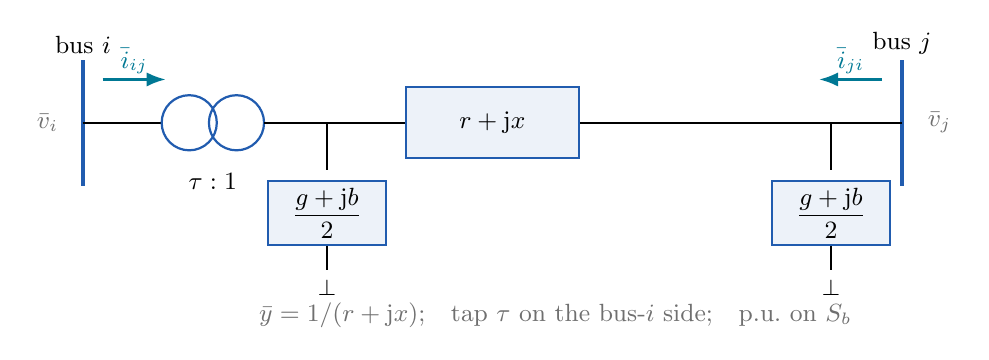
\begin{tikzpicture}[x=1cm,y=1cm]
  \draw[very thick, ethblue] (0,-0.1)   -- (0,1.5)  node[above, lbl, text=black] {bus $i$};
  \draw[very thick, ethblue] (10.4,-0.1) -- (10.4,1.5) node[above, lbl, text=black] {bus $j$};
  \node[port] at (-0.45,0.7) {$\bar v_i$};
  \node[port] at (10.88,0.7) {$\bar v_j$};
  % tap transformer
  \draw[wire] (0,0.7) -- (1.0,0.7);
  \draw[thick, ethblue] (1.35,0.7) circle (0.35);
  \draw[thick, ethblue] (1.95,0.7) circle (0.35);
  \node[lbl] at (1.65,-0.05) {$\tau : 1$};
  \draw[wire] (2.3,0.7) -- (3.5,0.7);
  % series impedance
  \node[block, minimum width=22mm] (z) at (5.2,0.7) {$r + \mathrm{j}x$};
  \draw[wire] (3.5,0.7) -- (z.west);
  \draw[wire] (z.east) -- (10.4,0.7);
  % shunts
  \draw[wire] (3.1,0.7) -- (3.1,0.1);
  \node[block, minimum width=15mm, minimum height=8mm] (shi) at (3.1,-0.45) {$\dfrac{g + \mathrm{j}b}{2}$};
  \draw[wire] (shi.south) -- ++(0,-0.3) node[below] {\footnotesize$\perp$};
  \draw[wire] (9.5,0.7) -- (9.5,0.1);
  \node[block, minimum width=15mm, minimum height=8mm] (shj) at (9.5,-0.45) {$\dfrac{g + \mathrm{j}b}{2}$};
  \draw[wire] (shj.south) -- ++(0,-0.3) node[below] {\footnotesize$\perp$};
  % current arrows
  \draw[sig, ethpetrol] (0.25,1.25) -- (1.05,1.25) node[midway, above, lbl, text=ethpetrol] {$\bar i_{ij}$};
  \draw[sig, ethpetrol] (10.15,1.25) -- (9.35,1.25) node[midway, above, lbl, text=ethpetrol] {$\bar i_{ji}$};
  % annotation
  \node[lbl, text=ethgrey] at (6.0,-1.75)
    {$\bar y = 1/(r+\mathrm{j}x)$;\quad tap $\tau$ on the bus-$i$ side;\quad p.u.\ on $S_b$};
\end{tikzpicture}
\end{document}
